\subsection{Optimizations for PPA}\label{sec:computingprobabilitiesOptimizations}

While model counting and solution space quantification are general problems, their application to probabilistic program analysis can often be improved exploiting the additional information specific to this application field.

We briefly report in this section two techniques able to 1) exploit variables dependency to reduce the complexity of model counting and solution space quantification and 2) combine interval constraint propagation and stratified sampling to increase the accuracy of sampling-based probability computation, and in turn its convergence rate.

\paragraph{Divide and conquer.}
The complexity of all the model counting and solution space quantification techniques proposed in this section depends on the number of variables involved in the constraints to be quantified. Let us assume such constraints are provided in disjunctive normal form and that there is no intersection between the solution spaces of any pair of disjuncts (this is form is quite natural for most constraints analyzed in PPA, usually requiring low computational overhead for normalization). Since there is no intersection between the disjuncts, the solution space for each of them can be quantified separately and than summed up to obtain the result for the whole disjunction.

Let us focus on a single disjunct $\phi \equiv \phi_1 \land \phi_2 \land \dots \land \phi_n$ predicating on the variables $\{v_1, v_2, \dots, v_m\}$, i.e., for each $v_i$ there exists at least one conjunct $\phi_j$ predicating on its value. Our goal is to divide the quantification of the solution space of $\phi$ in a set of independent problems involving only a subset of the variables appearing in $\phi$. 

The central idea is that constraints in $\phi$ identify a dependency relation ($\textit{dep}$) among the constrained variables that can be formalized as follows (let $v_i$, $v_j$, and $v_k$ be variables in $\phi$ and $\phi_i$ be a conjunct in $\phi$):
\begin{itemize}
	\item $\forall v_i \ \textit{dep}(v_i,v_i)$
	\item $\forall v_i,v_j$ if there exist a conjunct $\phi_i$ predicating on both $v_i$ and $v_j$, then $\textit{dep}(v_i,v_j)$
	\item $\forall v_i,v_j,v_k$ $\textit{dep}(v_i,v_j) \land \textit{dep}(v_j,v_k) \implies \textit{dep}(v_i,v_k)$
\end{itemize}

The intuitive meaning of the $\textit{dep}$ relation is that if $\textit{dep}(v_i,v_j)$ then the values assumed by $v_i$ in a program run affect the values that can be assumed by $v_j$ towards the satisfaction of $\phi$. For example, from $\{x>5 \land y=x+5\}$ we deduce that the value of $y$ is affected by the values of $x$, and vice versa. The relation $\textit{dep}$ is an equivalence relation, thus it induces a partition on the set of variables appearing in $\phi$. For this reason, we can rewrite $\phi$ as the conjunction of the subsets $\phi_{[v]}$, each of whom collects all the constraints involving a variable in the equivalence class of $\textit{dep}$ represented by $v$. Such conjuncts are logically separated, hence it can be proved that $\textit{Pr}(\phi)= \prod_{v} \textit{Pr}(\phi_{[v]})$. 

For example, let $\phi$ be $\{x>2 \land y<5\}$, its probability can be computed as $\textit{Pr}(\phi)=\textit{Pr}(x>2) \cdot \textit{Pr}(y<5)$. The computation of the two probabilities on the right-hand side of this equality can be performed independently and each of them involves only one variable, reducing the effort of counting in a multidimensional space or taking samples from multidimensional distributions. Furthermore, the result of each subproblem can be cached and reused, with significant benefits in practical applications~\cite{Filieri2013}.


\paragraph{Interval constraint propagation and stratified sampling.}
Despite their generality, sampling-based methods for computing probability may suffer slow convergence rate. Several techniques have been established in statistics to mitigate this general issue~\cite{Robert2005MCBook}. Besides these techniques, the specificity of the problems we face in PPA can be exploited to define even more effective variance reduction technique.

Recall the example we introduced in Section~\ref{sec:computingprobabilitiesSampling}: we aim at quantifying the probability of satisfying the constraint 
$v_1 \leq -v_2 \land v_2 \leq v_1$, where both $v_1, v_2 \in [-1, 1] \cap \mathbb{R}$. Figure~\ref{fig:stratifiedICP} shows the domain and the solution space for this problem, with $v_1$ on the x-axis and $v_2$ on the y-axis. Using hit-or-miss Monte Carlo to solve this problem requires throwing random samples for $v_1$ and $v_2$ within their domain (i.e., from within the square), and computing the ratio between those falling within the shadowed triangle (i.e., satisfying the constraints) and the total number of samples. Geometrically, this corresponds to estimating the ratio between the area of the triangle and the area of the square (which is 1/4).

\begin{figure}[h!]\label{fig:stratifiedICP}
  \centering
      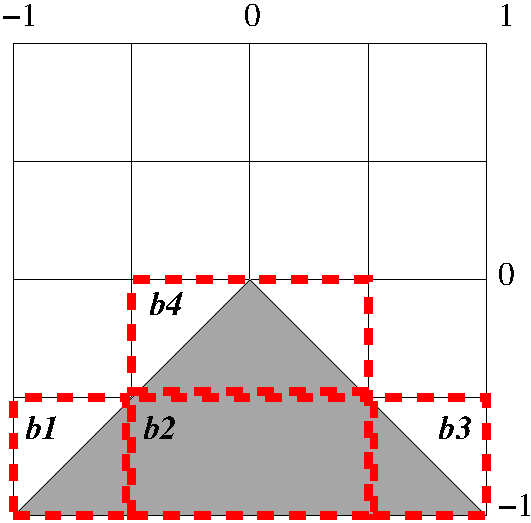
\includegraphics[width=3cm]{triangle}
  \caption{Example of ICP-based domain partitioning.}
\end{figure}

Looking at the figure it is evident that some regions of the domain do not contain solutions, i.e., the probability of satisfying the constraint within those regions is identically 0, without any estimation uncertainty. Intuitively, since we have an exact information about a fraction of the domain, we can confine the estimation, and consequently the uncertainty of estimation, only on the remaining part of the domain. This intuition can be systematized combining two techniques: interval constraint propagation and stratified sampling. 

Interval constraint propagation (ICP) is a algorithmic technique to compute interval solutions to equality and inequality numerical constraints. The input of ICP is a set of $n$ variables, each one defined on a convex domain, and a conjunction of numerical constraints; its output is a set of $n$-dimensional non-overlapping boxes whose union contains all the values of the variables satisfying all the constraints. Each box is essentially an hyperplane bounding a portion of the domain that contains solutions for the problem plus, possibly, other points that do not satisfy the constraint. Looking again at Figure~\ref{fig:stratifiedICP}, the application of ICP to our constraint produces the four 2-dimensional red boxes, whose union contains all the solutions. ICP can thus be used to partition the input domain into a set of regions, where each region may 1) contain no solutions, 2) contain only solutions, or 3) contain both solutions and values that do not satisfy the constraint. In the first two cases computing the probability will trivially lead to 0 and 1, respectively, without any uncertainty (i.e., zero variance). In the third case, sampling is needed to estimate the fraction of solution points.

When we have local results for each region in the domain partition, the second step is to compose these local information to obtain the probability estimate for the whole domain. Stratified sampling is a statistical techniques allowing to compose the local estimators of each region of the domain into a global estimator for the initial problem~\cite{Robert2005MCBook}. This computation is essentially a weighted sum of the local estimators, where the weight is the size of the region divided by the size of the domain. If we call $\hat{P}_i$ the local estimator of the $i$-th region and $w_i$ the ratio between the size of the $i$-th region and the size of the domain, exploiting the properties of expected value and variance for a sum of independent random variables~\cite{pestman1998mathematical}, we obtain for the global estimator $\hat{P}$ the following properties:

\begin{equation}\label{eq:stratifiedSampling}
	E[\hat{P}]=\sum_i w_i \cdot E[\hat{P}_i] \qquad Var[\hat{P}] = \sum_i w_i^2 \cdot Var[\hat{P}_i]
\end{equation}

The variance for the regions containing no solutions is trivially 0, thus the variance of the global estimator is reduced by the squared weight of these regions. Furthermore, for regions containing only solutions, the sampling-based probability computation will return variance 0 as well (recall Equation~\eqref{eq:mleEstimator}). Thus, fixed the total number of samples, the uncertainty on the global estimator with stratified sampling is always smaller or equal than the one we can obtain by applying Monte Carlo estimation on the whole domain, without partitions (this is a general result for stratified sampling~\cite{Robert2005MCBook}). 

The effectiveness of this approach depends on how much of the domain can be pruned out by the adopted ICP technique. This approach has been implemented in~\cite{Borges2014}, using the open-source ICP solver RealPaver~\cite{granvilliers2006tomas} for floating-point constraints, showing a significant reduction of the estimator variance on several realist programs, and, in turn, a faster convergence rate of the sampling-based probability computation. A combination of this technique with the previous divide and conquer strategy has been further developed in~\cite{2015-fse-qcoral} for a finer focusing of the sampling effort on the constraints and regions mostly affecting the variance of the global estimator, obtaining even faster convergence rates.





